\documentclass[a4paper,11pt]{article}
\usepackage[utf8x]{inputenc}
\usepackage{a4wide}
\usepackage[spanish,activeacute]{babel}
\usepackage{graphicx}
\usepackage{float}
\usepackage{listings}
\usepackage{placeins}
\usepackage[colorlinks,citecolor=black,filecolor=black,linkcolor=black,    urlcolor=black]{hyperref}
\usepackage{enumitem}
\floatstyle{boxed}
\newfloat{tarea}{thpH}{lop}
\floatname{tarea}{Lote}

\lstdefinelanguage{JavaScript}{
  keywords={typeof, new, true, false, catch, function, return, null, catch, switch, var, if, in, while, do, else, case, break},
  %keywordstyle=\color{blue}\bfseries,
  ndkeywords={class, export, boolean, throw, implements, import, this},
%  ndkeywordstyle=\color{darkgray}\bfseries,
  identifierstyle=\color{black},
  sensitive=false,
  comment=[l]{//},
  morecomment=[s]{/*}{*/},
  morestring=[b]',
  morestring=[b]"
}

\begin{document}
\lstset{language=JavaScript}
\lstset{ %
  basicstyle=\small
}

\markboth{left head}{Sistemas Operativos 2014 -- TP N\textordmasculine 3}
\pagestyle{myheadings}

\title{
	\mbox{\Huge Universidad de Buenos Aires}\\
	\mbox{\LARGE Facultad de Ciencias Exactas y Naturales}\\
	\mbox{\LARGE Departamento de Computación}\\
	\mbox{\LARGE Sistemas Operativos}\\
	\mbox{Trabajo Práctico Número 3}\\
}

\date{}

\maketitle

\thispagestyle{empty}

\begin{center}
	\begin{tabular}{c}
		\hline
		\\
		Primer Cuatrimestre de 2014\\
		\\
		\hline
		\\
		\\
	\end{tabular}

	\begin{tabular}{|l|r|l|}
		\hline
		\textbf{Nombre} & \textbf{L.U.} & \textbf{e-mail}\\
		\hline
		Emilio Almansi & 674/12 & \verb"ealmansi@gmail.com"\\
		\hline
		Jose Fernando Alvaro & 089/10 & \verb"fer1578@gmail.com"\\
		\hline
		Sebastián Sgariglia & 721/95 & \verb"ssgariglia@gmail.com"\\
		\hline
	\end{tabular}
\end{center}

\vskip 5mm




\clearpage
\tableofcontents

\clearpage
\section{Introducción}

Con la motivación de estudiar el problema de almacenar y analizar grandes cantidades de datos, dentro del área que se conoce como \emph{Big Data}, contamos con una base de datos de más de medio millón de reseñas reales de la tienda virtual de \emph{Amazon}. Las reseñas son acerca de películas comercializadas en el sitio, habiendo sido escritas por usuarios reales; cada una contiene varios campos de información, entre ellos un identificador del producto sobre el que se hace referencia (\textbf{productId}), el puntaje que asignó el usuario a la película (\textbf{score}), un índice de valoración de la reseña según otros usuarios del sitio (\textbf{helpfulness}), o el texto completo con la opinión del autor (\textbf{text}).

En una primera etapa, realizamos un análisis sobre los datos con la finalidad de obtener la siguiente información: cuáles son las películas mejor rankeadas (según el \textbf{score} de las reseñas), cuáles son las palabras más utilizadas para opinar sobre los productos en función del puntaje que asignó el autor, y cuál es la relación entre la longitud de las reseñas y el índice de valoración que han recibido. Esto se realizó siguiendo el esquema \emph{MapReduce}, implementando las funciones \textbf{map}, \textbf{reduce} y opcionalmente \textbf{finalize} para cada una de las preguntas que se deseaba responder.

Finalmente, estudiamos la escalabilidad de la solución propuesta, de forma tal de poder almacenar una cantidad creciente de datos, manteniendo a su vez el tiempo requerido para el análisis de los mismos dentro de rangos aceptables.
\section{Análisis de los datos}

A continuación detallamos la implementación de las funciones para cada uno de los análisis pedidos:

\subsection{Punto 1}

Encontrar las doce películas mejor rankeadas de la colección de reseñas con al menos veinte reseñas.

\subsubsection{Descripción}

Función \textbf{map}:\\\\
En este paso emitimos como key al \emph{productId} del documento (que identifica a la película), y como \emph{value} un objeto con las siguientes propiedades:

\begin{description}
	\item[count:] cantidad de reseñas.
	\item[score:] puntaje otorgado a la película por el reviewer.
\end{description}

\begin{lstlisting}[frame=leftline]
  function() {
    key = this.productId;
    value = { 
      count: 1,                       // ocurrences
      score: parseInt(this.score,10)  // score
    };
    emit(key, value);
  }
\end{lstlisting}

Función \textbf{reduce}:\\\\
En este paso se acumula la cantidad total de reseñas en la propiedad \textbf{count} y la suma de todos los puntajes en la propiedad \textbf{score}:

\begin{lstlisting}[frame=leftline]
  function (key, values) {
    reducedValue = {
      count: 0,
      score: 0,
    };
    for (var i=0; i < values.length; i++){
      reducedValue.count += values[i].count;	// total ocurrences
      reducedValue.score += values[i].score;	// total score
    }
    return reducedValue;
  }
\end{lstlisting}

Función \textbf{finalize}:\\\\
Como queremos considerar sólo las películas con al menos veinte reseñas, hacemos uso de esta función con el siguiente código:\\

\begin{lstlisting}[frame=leftline]
  function (key, reducedValue) { 
    if(reducedValue.count >= 20){
      return reducedValue.score/reducedValue.count;	// average score
    }
    else{
      return 0;
    }
  }
\end{lstlisting}

Donde si la cantidad de reseñas es mayor o igual a 20, devolvemos el promedio de las mismas dividiendo el score total por la cantidad de reseñas, caso contrario devolvemos 0.

\subsubsection{Resultado}

Para la obtención de los datos pedidos modificamos el archivo \textit{runner.py} para que guarde la ejecución de \textbf{mapreduce} en una nueva colección llamada ``ej1'' y luego le pida a \textit{mongo} que ordene los resultados en forma decreciente respecto al valor obtenido y nos devuelva los primeros 12 resultados solamente.\\

\begin{lstlisting}[frame=leftline]
getattr(db,outcoll).aggregate([{"$sort":SON([("value",-1)])},
  {"$limit":12},{"$out":outcoll}])
coll = getattr(db,outcoll).find()
print "Los producId de las 12 peliculas mejor rankeadas en amazon son (",
for res in coll:
	print res['_id'],
print ")"
\end{lstlisting}

Los resultados obtenidos fueron los siguientes:
\begin{enumerate}
\item B0002NY7UY : Live in Concert [VHS]
\item B0007GAEXK : The Mole - The Complete First Season (2001)
\item B00000JSJ5 : All Creatures Great and Small, Series 2: Volumes 1-6 [VHS] (1990)
\item B0007Z4HAC : Salsa Crazy Presents: Learn to Salsa Dance, Intermediate Series, Volume 1 (2005)
\item B000AOEPU2 : WWE: Bret "Hitman" Hart - The Best There Is, The Best There Was, The Best There Ever Will Be (2005)
\item B00004YKS7 : Genghis Blues (1999)
\item B00004YKS6 : Genghis Blues [VHS] (1999)
\item B000MCIADA : A Reiki 1st, Aura and Chakra Attunement Performed (2007)
\item B008COIZHQ : Genghis Blues 1999
\item B006JN87UC : Transformers: Prime - Season One (Limited Edition) [Blu-ray] (2012)
\item B003YBGJ4S : WELL worked out with Tannis
\item B004LK24BI : 50/50 Cardio and Weights with Angie Gorr (2011)
\end{enumerate}


\subsection{Punto 2}
Por cada puntaje de review (1-5) encontrar las palabras más frecuentes en sus respectivas reseñas sin contar stop words.

\subsubsection{Descripción}

Función \textbf{map}:\\\\
En este paso tomamos el texto de la review y lo separamos en tokens obteniendo un array de palabras. A su vez disponemos de un array de stopwords que usaremos a continuación. Si el array de palabras del review no es vacío, tomamos cada palabra y removemos sus caracteres no alfanuméricos. Luego si la palabra no corresponde a un stopword le asignamos un 1 al nivel de score que corresponde a la reseña en cuestión. Para ello se utiliza un objeto que contiene un contador para cada nivel de score como propiedad. Luego emitimos este objeto como value con la palabra en cuestión como key:

\begin{lstlisting}[frame=leftline]
  function() {
    var stopwords = [...];
    var words = this.text.split(" ");	//array of words from text
    if (words) {
      //not empty array
      for (var i=0; i < words.length; i++) {
        //words in lower case, without punctuation and special chars
        var word = words[i].toLowerCase().replace(/[^a-zA-Z 0-9]+/g,'');
        if (stopwords.indexOf(word) == -1 && word){	
          //not stop word or empty word
          value = {s1: 0, s2: 0, s3: 0, s4: 0, s5: 0};	// count for each score
          var index = this.score;
          if (index == 1) {
            value.s1 = 1;
          }				
          else if(index == 2){
            value.s2 = 1;
          }
          else if(index == 3){
            value.s3 = 1;
          }
          else if(index == 4){
            value.s4 = 1;
          }
          else{
            value.s5 = 1;
          }
          emit(word,value);
        }
      }
    }
  }
\end{lstlisting}

Functión \textbf{reduce}:\\\\
En este paso se acumula para cada palabra emitida la cantidad de ocurrencias en cada nivel de score:

\begin{lstlisting}[frame=leftline]
  function (key, values) { 
    reducedValue = {s1: 0, s2: 0, s3: 0, s4: 0, s5: 0};
    for(var i=0; i < values.length; i++) {	//total occurrences for words
      reducedValue.s1 += values[i].s1;
      reducedValue.s2 += values[i].s2;
      reducedValue.s3 += values[i].s3;
      reducedValue.s4 += values[i].s4;
      reducedValue.s5 += values[i].s5;
    }
    return reducedValue;
  }
\end{lstlisting}

\subsubsection{Resultado}

Para la obtención de los datos pedidos modificamos el archivo \textit{runner.py} para que guarde la ejecución de \textbf{mapreduce} en una nueva colección llamada ``ej2'' y luego le pida a \textit{mongo} que por cada valor de ``score'' ordene los resultados en forma decreciente respecto al valor obtenido y nos devuelva los primeros 5 resultados solamente.\\

\begin{lstlisting}[frame=leftline]
getattr(db,outcoll).aggregate([{"$out" : outcoll}])
for i in range(1,6):
	coll = getattr(db,outcoll).find().sort("value.s" + str(i),-1).limit(5)
	print u"Las 5 palabras mas frecuentemente usadas con score = %s son (" % i,
	for res in coll:
		print "%s" % res['_id'],
	print ")"
\end{lstlisting}

Los resultados obtenidos fueron los siguientes:

\begin{enumerate}
\item Las 5 palabras mas  usadas con score = 1 son: movie, one, film, dvd, even
\item Las 5 palabras mas  usadas con score = 2 son: movie, film, one, good, dvd 
\item Las 5 palabras mas  usadas con score = 3 son: movie, film, good, one, dvd 
\item Las 5 palabras mas  usadas con score = 4 son: movie, film, good, one, great
\item Las 5 palabras mas  usadas con score = 5 son: movie, one, great, film, dvd 
\end{enumerate}

\subsection{Punto 3}

Por cada puntaje de helpfulness, calcular la longitud promedio del review text.

\subsubsection{Descripción}

Función \textbf{map}:\\\\
En este paso tomamos el texto de la review y asignamos su longitud a la propiedad \textbf{len} del objeto value a devolver, además de poner su propiedad \textbf{count} en 1. Luego emitimos este objeto con el puntaje de helpfulness como key.

\begin{lstlisting}[frame=leftline]
  function() {
    var text = this.text;
    var find = "<br />";
    var regex = new RegExp(find, "g");
    text = text.replace(regex, ""); // remove <br />
    value = { 
      count: 1, 
      len: text.length 
    };
    var parts = this.helpfulness.split("/");
	parts[0] = parseFloat(parts[0]);
	parts[1] = parseFloat(parts[1]);
	if (parts[1] != 0 && parts[0] <= parts[1])
		emit((parts[0] / parts[1]).toFixed(4),value);	//key as number
  }
\end{lstlisting}

Functión \textbf{reduce}:\\\\
En este paso acumulamos para cada puntaje de helpfulness el total de ocurrencias de ese puntaje y la longitud de los reviews correspondientes:

\begin{lstlisting}[frame=leftline]
  function (key, values) {
    reducedValue = { 
      count: 0, 
      len: 0 
    }; 
    for(var i=0; i < values.length; i++){
      reducedValue.count += values[i].count;  // total occurences
      reducedValue.len += values[i].len;      // total text length
    }
    return reducedValue;
  }
\end{lstlisting}

Functión \textbf{finalize}:\\\\
Aquí realizamos el cálculo del promedio de la longitud del texto para cada puntaje de helpfulness.

\begin{lstlisting}[frame=leftline]
  function (key, reducedValue){
    return reducedValue.len / reducedValue.count; // average text length
  }
\end{lstlisting}

\subsubsection{Resultado}

Para la obtención de los datos pedidos modificamos el archivo \textit{runner.py} para que guarde la ejecución de \textbf{mapreduce} en una nueva colección llamada ``ej3'' y luego le pida a \textit{mongo} que nos devuelva los resultados obtenidos.\\

\begin{lstlisting}[frame=leftline]
getattr(db,outcoll).aggregate([{"$out" : outcoll}])
coll = getattr(db,outcoll).find()
for res in coll:
	print "helpfulness:",
	print res['_id'],
	print ", average length:",
	print res['value'] 
\end{lstlisting}

A modo de ejemplo mostraremos los primeros 10 resultados obtenidos: 

\begin{enumerate}
\item helpfulness: 0.0 , average length: 434.590073212
\item helpfulness: 0.00401606425703 , average length: 429.0
\item helpfulness: 0.00680272108844 , average length: 248.0
\item helpfulness: 0.00819672131148 , average length: 200.0
\item helpfulness: 0.00917431192661 , average length: 388.0
\item helpfulness: 0.0102040816327 , average length: 418.0
\item helpfulness: 0.0103092783505 , average length: 514.0
\item helpfulness: 0.0108695652174 , average length: 755.0
\item helpfulness: 0.0111111111111 , average length: 277.0
\item helpfulness: 0.0113636363636 , average length: 490.5
\end{enumerate}


\subsection{Punto 4}

A partir del resultado del punto 3, calcular la correlación entre ambas magnitudes.

\subsubsection{Descripción}

Como fuese indicado por la catedra la medida de correlación que calcularemos es el coeficiente de correlación de \textbf{Pearson}.
El coeficiente de correlación de \textbf{Pearson} es una medida de correlación o dependencia entre 2 variables. El mismo varia en los valores ``+1'' y ``-1'' donde una valor ``1'' implica una correlación totalmente positiva, un valor de ``0'' implica que no hay correlación y un valor de ``-1'' implica una correlación totalmente negativa.

\subsubsection{Resultado}

Para la obtención de los datos pedidos modificamos el archivo \textit{runner.py} para que cuando corra la ejecución del ejercicio 3 guarde los datos de ``helpfulness'' y ``length'' en 2 array los cuales luego pasamos a una función que calcula el coeficiente de correlacion de \textbf{Pearson}. A su vez tambien genera el plot de los datos cuando es llamado con el argumento ``--plot''.

\begin{lstlisting}[frame=leftline]
getattr(db,outcoll).aggregate([{"$out" : outcoll}])
coll = getattr(db,outcoll).find()
help = []
length = []
for res in coll:
	print "helpfulness:",
	print res['_id'],
	help.append(float(res['_id']))
	print ", average length:",
	print res['value'] 
	length.append(res['value'])
	print
	print "The Pearson correlation is: %s" % pearson_def(help,length)
		if(args.plot):
		plot(help,length)
\end{lstlisting}

\begin{figure}[H]
  \centering
  \makebox[\textwidth][c]{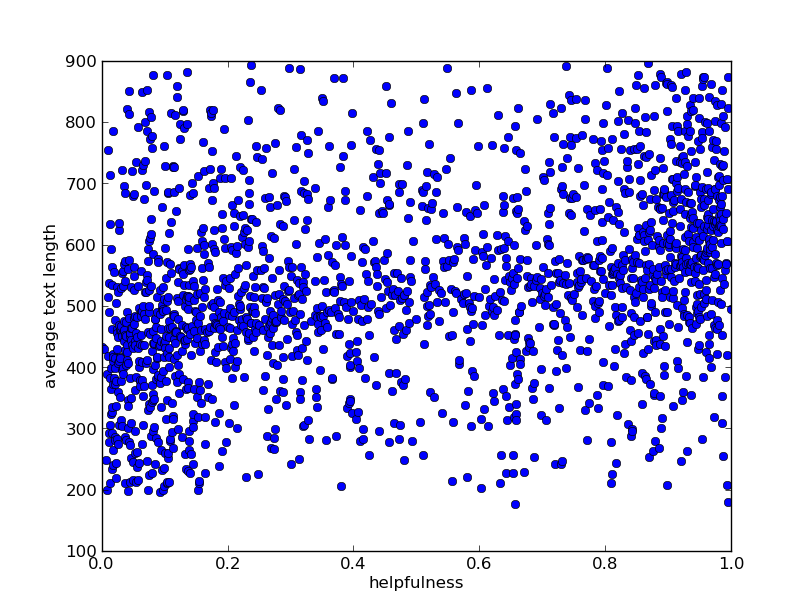
\includegraphics[width=0.70\textwidth]{ej4.png}}%
  \caption{Helpfulness y Length para los datos del ejercicio 3}
  \label{fig41}
\end{figure}

Con los datos del grafico de la figura~\ref{fig41}, el coeficiente de correlación de \textbf{Pearson} obtenido fue de: \textbf{0.322148330724}

\subsubsection{Conclusión}

Dado que el coeficiente de correlación de \textbf{Pearson} es igual a 0.322148330724, podemos concluir que existe cierto grado de correlación positiva entre el puntaje de ``Helpfulness'' y la longitud del texto de la reseña.
Puede observarse en el grafico de la figura~\ref{fig41} que la gran mayoria de los textos tienen una longitud promedio de alrededor de 500 caracteres y son los menos valorados. Se nota tambien cierta tendiencia que al aumentar la longitud del texto aumenta tambien el nivel de valoración.

\section{Análisis de escalabilidad}

Para la base de datos de prueba (de unos $4GB$ aproximadamente), el análisis de las palabras más frecuentes ya requiere un tiempo de cómputo de varios minutos utilizando una única computadora; un crecimiento constante en el volúmen de datos solo puede empeorar la perfomance. Por esto mismo, para reducir los requerimientos de almacenamiento y mejorar la performance de una forma escalable, es necesario realizar el cómputo de forma distribuída.

El esquema \emph{MapReduce} se desarrolló específicamente para resolver este problema, permitiendo paralelizar de forma natural el procesamiento de los datos entre las múltiples computadoras de un cluster. En este caso en particular, si las reseñas de la base de datos se encuentran repartidas entre múltiples servidores, cada uno de ellos tiene menores requerimientos de almacenamiento, y puede procesar la función \textbf{map} sobre cada una de sus reseñas independientemente de las demás. Adicionalmente, cada servidor puede ejecutar la función \textbf{reduce} sobre los valores obtenidos, realizando reducciones parciales sobre los datos que tiene al alcance.

Esta técnica de distribución de los datos se conoce como \emph{Sharding}\footnote{http://docs.mongodb.org/manual/core/sharding-introduction/}. Es posible almacenar una base de datos a lo largo de múltiples servidores virtuales, utilizando un motor de base de datos como \emph{MongoDB} y una plataforma tipo \emph{IaaS} que provea flexibilidad cuando sea necesario escalar el volúmen de datos o mejorar la performance de las consultas.

\subsection{Amazon EC2}

\emph{Amazon EC2 (Elastic Compute Cloud)} fue de las primeras plataformas \emph{IaaS} en aparecer y se mantiene como una de las más avanzadas. Provee un enorme abanico de posibilidades para la creación, configuración y monitoreo de máquinas virtuales o \emph{AMI}s (\emph{Amazon Machine Instance}). Se comienza seleccionando un tipo de instancia según la cantidad de virtual cores, memoria, espacio en disco y velocidad del core que se necesite. Las instancias puede correr varios sistemas operativos, incluyendo Windows, Linux, etc, y se puede elegir entre instancias ya predefinidas o construir una propia. Cada instancia puede correrse en datacenters diferentes, ubicados en distintas regiones geográficas. Esto puede utilizarse para seleccionar la región con menor latencia o establecer un criterio de redundancia ante cualquier problema con una región específica.

Una ventaja adicional de \emph{Amazon EC2} es el hecho de que hay abundante bibliografía sobre cómo establecer bases de datos (utilizando \emph{MongoDB} por ejemplo) de forma escalable, utilizando máquinas virtuales con \emph{Linux}.\footnote{http://docs.mongodb.org/ecosystem/platforms/amazon-ec2/}

Una opción para mantener los datos de las reseñas y procesar las consultas en tiempos razonables podría ser mantener múltiples instancias medianas \emph{On Demand}\footnote{http://aws.amazon.com/ec2/pricing/}:

\begin{verbatim}
              vCPU  ECU Memory (GiB)  Instance Storage (GB) Linux/UNIX Usage
  m3.medium   1     3   3.75          1 x 4 SSD             $0.070 per Hour
\end{verbatim}

Las mismas se cobran solo por el tiempo en que son efectivamente utilizadas, permitiendo alternar la cantidad de instancias en función de los requerimientos de uso, así como extender el volúmen de datos cuando sea necesario.

Sin embargo, si se puede estimar con precisión el ritmo de crecimiento del volúmen de datos o nivel de uso (por ejemplo, un cierto porcentaje anual), una mejor opción sería tomar instancias por tiempo determinado. 

En el caso de tomar instancias medianas por períodos anuales\footnote{http://aws.amazon.com/ec2/pricing/}:

\begin{verbatim}
              Upfront Hourly         
  m3.medium   $110    $0.064 per Hour
\end{verbatim}

Esto reduce ampliamente los costos, pero a la vez permite incrementar el número de instancias al término del período.

\subsection{Linode}

Linode es un respetado proveedor de VPSs o virtual private servers con Linux. Ofrece diversos planes que se diferencian con respecto a la cantidad de RAM del servidor, la cantidad de cores asignados, los límites de espacio en disco y tranferencia de datos mensuales. La elección de cada plan conlleva un gasto mensual fijo, se usen o no los recursos disponibles en el plan contratado. 

Linode cuenta con 6 datacenters en 3 regiones (continentes) diferentes, pudiendo elegir el datacenter en la región que brinda los menores tiempos de latencia (proveen una página de testing para ello). También dispone de un panel de control a través del cual se puede manejar el ciclo de vida de las máquinas virtuales, y un API para realizar tareas administrativas en forma programática. Para crear una máquina virtual sólo debe elegirse la distribución requerida y se procede a instanciarla con el acceso a los recursos ofrecidos por el plan elegido.

Otros servicios que ofrecen son administración del DNS de cada nodo, monitoreo, backup, y balanceo de datos entre un cluster de nodos en caso de necesitar tales configuraciones (con diferentes características de configuración, tales como sticky sessions, chequeo dinámico de servidores activos, etc). Varios de estos servicios con costo aparte.


\end{document}
